
\setcounter{chapter}{1}
\chapter{Conception}
\minitoc %insert la minitoc
\graphicspath{{Chapitre2/figures/}}

%\DoPToC

%==============================================================================
\pagestyle{fancy}
\fancyhf{}
\fancyhead[R]{\bfseries\rightmark}
\fancyfoot[R]{\thepage}
\renewcommand{\headrulewidth}{0.5pt}
\renewcommand{\footrulewidth}{0pt}
\renewcommand{\chaptermark}[1]{\markboth{\MakeUppercase{\chaptername~\thechapter. #1 }}{}}
\renewcommand{\sectionmark}[1]{\markright{\thechapter.\thesection~ #1}}

\begin{spacing}{1.2}
%==============================================================================

\section*{Introduction}
Vu que nous avons achevé la première phase (Analyse) du cycle de développement, nous aborderons dans ce chapitre la deuxième phase (Conception) qui se concentre essentiellement sur la définition de l’architecture du système ainsi que sur l’analyse et la conception des besoins et des exigences des utilisateurs.  L’activité d’analyse et de conception permet de traduire les besoins fonctionnels et les contraintes issues du cahier des charges et de la spécification des exigences dans un langage plus professionnel et compréhensible par tous les individus intervenants dans la réalisation et l’utilisation de l’application

\newpage
\section{Diagrammes}
\subsection{Diagramme de cas d'utilisation}
Le diagramme de cas d'utilisation ( \autoref{fig:fig2} ) est utilisé pour donner une vision globale du comportement fonctionnel du système .

\begin{figure}[H]\centering
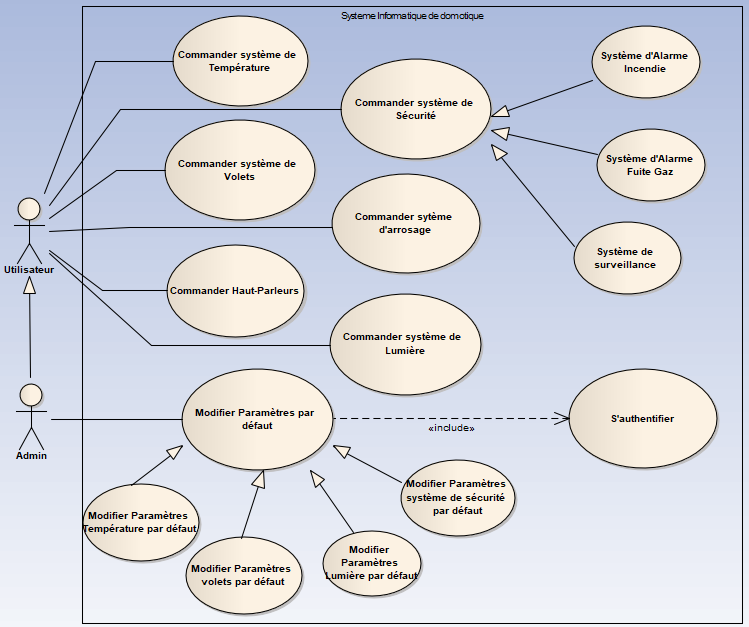
\includegraphics[scale=0.9]{1.png}
\caption{Diagramme de cas d'utilisations}
\label{fig:fig2}
\end{figure}




\begin{table}[H]
	\centering
	\caption{Classement des cas d’utilisation}
	\footnotesize
	\begin{tabularx}{\linewidth}{|>{\bfseries \vspace*{\fill}}X ||>{\centering{}\vspace*{\fill}}X|>{\vspace*{\fill}}X<{\centering{}}|}	
			\hline 
			Cas d’utilisation & \bfseries Priorité & \bfseries Risque\\
			\hline \hline
			Commander Système de Température		&	Moyenne	&	Moyen	\\
			Commander Système de Lumière		&	Moyenne	&	Moyen	\\
			Commander Système des Volets		&	Moyenne	&	Moyen	\\
			Commander Système de Sécurité		&	Moyenne	&	Moyen	\\
			Commander Système d’arrotissage		&	Moyenne	&	Moyen	\\
			Commander Haut-Parleurs		&	Faible	&	Moyen	\\
			Paramétrer Système de Sécurité		&	Haute	&	Haut	\\
			Paramétrer les Volets		&	Haute	&	Bas	\\
			Paramétrer la Lumière		&	Haute	&	Bas	\\
			Paramétrer la Température		&	Haute	&	Bas	\\
			S’authentifier		&	Faible	&	Haut	\\
			\hline
	\end{tabularx}
	\label{tab:exple}
\end{table}


\subsection{Diagrammes de Classes}
\subsubsection{Système de Température}

\begin{figure}[H]\centering
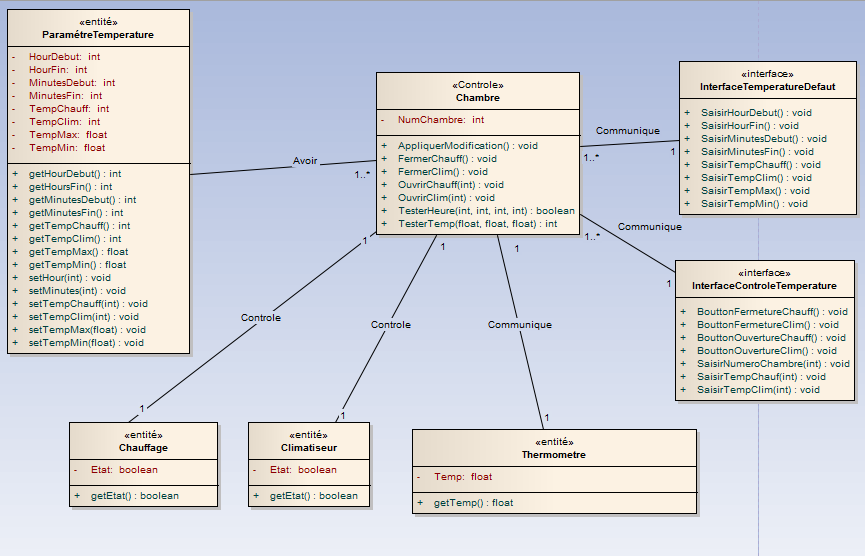
\includegraphics[scale=0.8]{2.png}
\caption{Diagramme de Classes du Système de Température}
\label{fig:fig3}
\end{figure}

\subsubsection{Système de Sécurité}

\textbf{Système de caméra de surveillance}

\begin{figure}[H]\centering
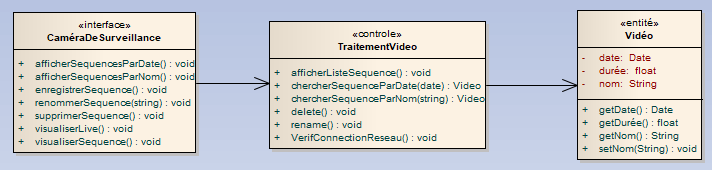
\includegraphics[scale=0.9]{3.png}
\caption{Diagramme de Classes du Système de caméra de surveillance}
\label{fig:fig3}
\end{figure}

\textbf{Système d’alarme d’incendie}

\begin{figure}[H]\centering
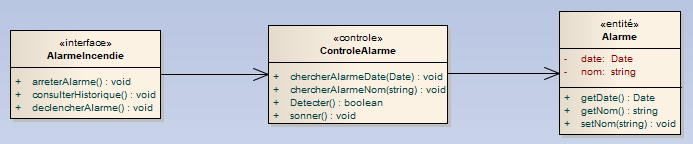
\includegraphics[scale=0.9]{4.png}
\caption{Diagramme de Classes du Système d’alarme d’incendie}
\label{fig:fig3}
\end{figure}

\textbf{Système d’alarme de fuite de Gaz}

\begin{figure}[H]\centering
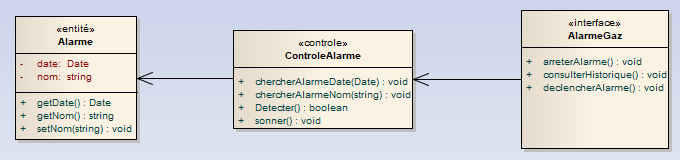
\includegraphics[scale=0.9]{5.png}
\caption{Diagramme de Classes du Système d’alarme de fuite de Gaz}
\label{fig:fig3}
\end{figure}

\subsubsection{Système de Volets}
\begin{figure}[H]\centering
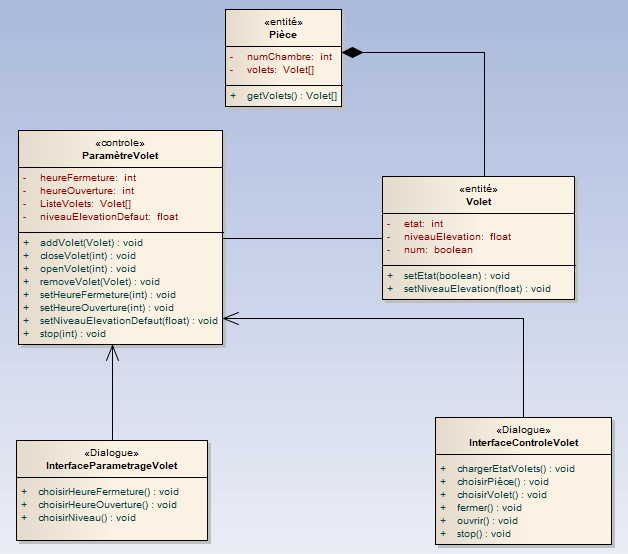
\includegraphics[scale=0.9]{6.png}
\caption{Diagramme de Classes du Système de Volets}
\label{fig:fig3}
\end{figure}

\subsubsection{Système de Lumière}
Remarques concernant quelques méthodes du diagramme de classe :
\begin{itemize}
    \item \textbf{debutCompteur :int} c’est la valeur du compteur à partir de laquelle on calcule la consommation d’électricité. 
    \item \textbf{gererConflit() :void} permet la gestion des problèmes si deux éclairages sont contradictoires et propose des suggestions de solutions. 
    \item \textbf{calculerConsommation() :void} permet de calculer la consommation , en effet  elle applique la formule suivante : consommation = numeroCompteur – debutCompteur. \\
    \item \textbf{indiquerFacturePayé () : void} permet d’informer le système que l’utilisateur a payé la facture d’électricité ce qui permet de calculer la consommation en électricité à partir du dernier péage.
    \item \textbf{CalculerDebutCompteur() :void} permet de changer l’attribut debutCompteur par le numero du compteur après un péage.
\end{itemize}

\begin{figure}[H]\centering
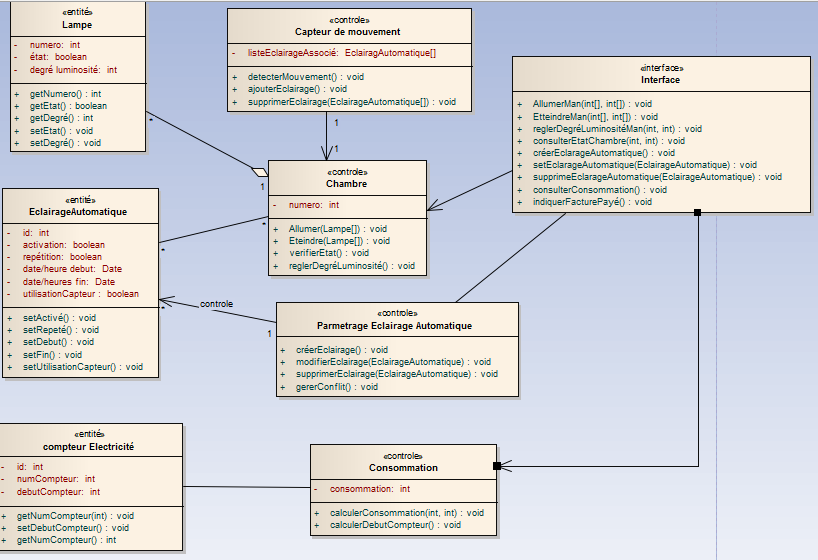
\includegraphics[scale=0.8]{7.png}
\caption{Diagramme de Classes du Système de Lumière}
\label{fig:fig3}
\end{figure}
 
\subsubsection{Système d’arrosage}
\begin{figure}[H]\centering
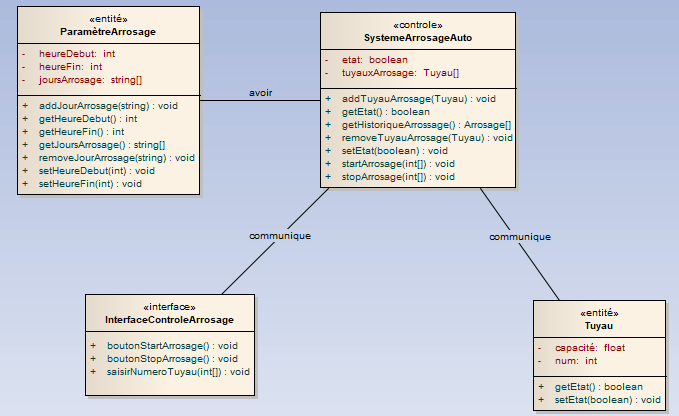
\includegraphics[scale=0.8]{8.png}
\caption{Diagramme de Classes du Système d’arrosage}
\label{fig:fig3}
\end{figure}

\subsubsection{Haut-Parleurs}
\begin{figure}[H]\centering
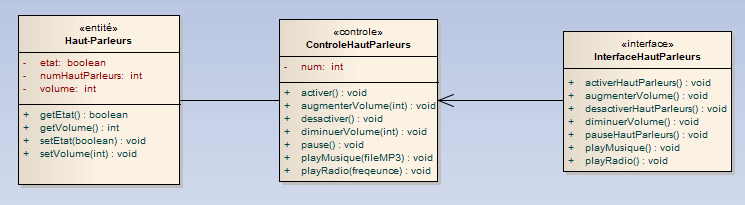
\includegraphics[scale=0.8]{9.png}
\caption{Diagramme de Classes des Haut-Parleurs}
\label{fig:fig3}
\end{figure}

\subsection{Diagramme de Paquetages}

\begin{figure}[H]\centering
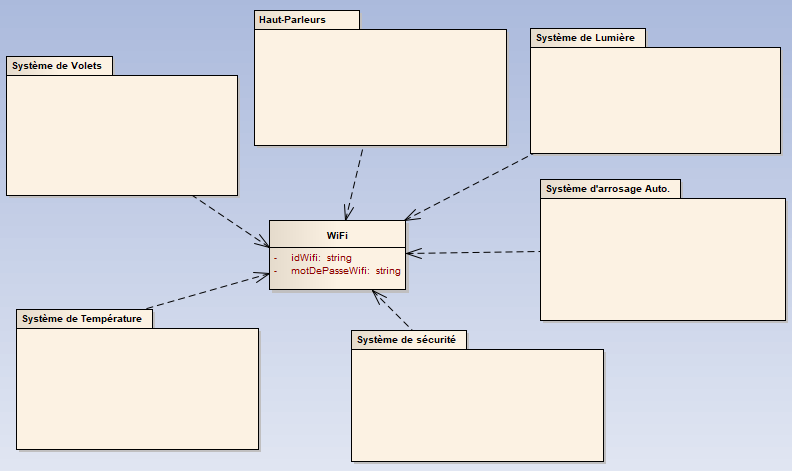
\includegraphics[scale=0.8]{32.png}
\caption{Diagramme de Paquetages}
\label{fig:fig3}
\end{figure}

\newpage

\subsection{Diagrammes de séquence}

\subsubsection{Système de température }

\textbf{Scénario de gestion automatique de la température : }
\begin{figure}[H]\centering
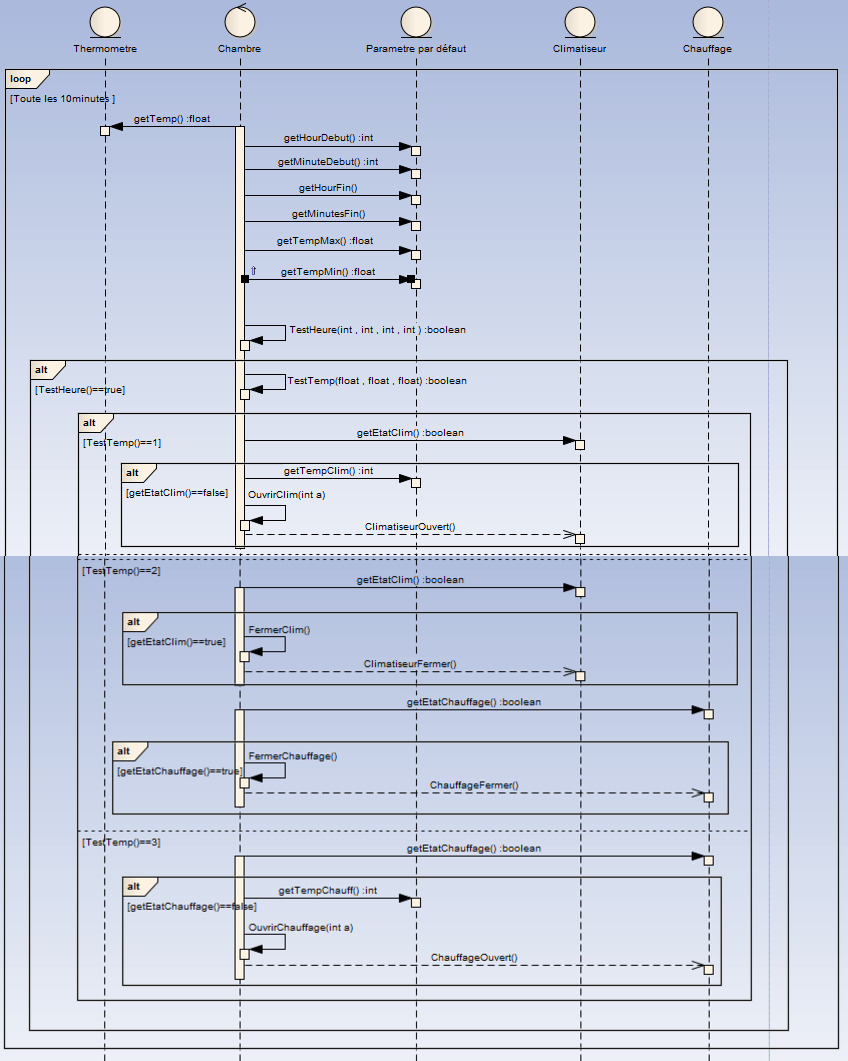
\includegraphics[scale=0.6]{12.jpg}
\caption{Diagramme de Séquence: Gestion automatique de la température}
\label{fig:fig3}
\end{figure}

\bigskip

\textbf{Scénario ouverture climatiseur manuelle : }
\begin{figure}[H]\centering
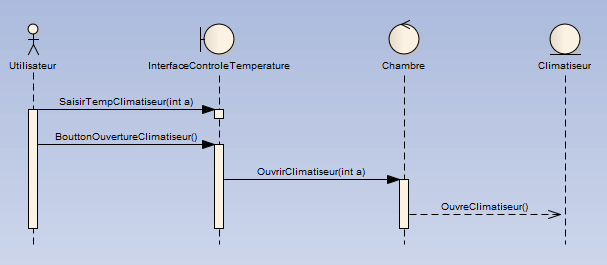
\includegraphics[scale=0.8]{13.png}
\caption{Diagramme de Séquence: Ouverture climatiseur manuelle}
\label{fig:fig3}
\end{figure}

\textbf{Scénario ouverture chauffage manuelle :}
\begin{figure}[H]\centering
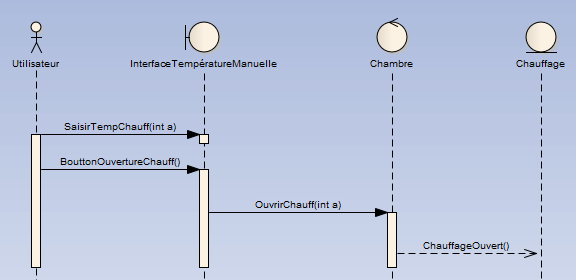
\includegraphics[scale=0.8]{14.png}
\caption{Diagramme de Séquence: Ouverture chauffage manuelle}
\label{fig:fig3}
\end{figure}

\newpage

\subsubsection{Système de lumière}

\textbf{Scénario d’éclairage manuel :}
\begin{figure}[H]\centering
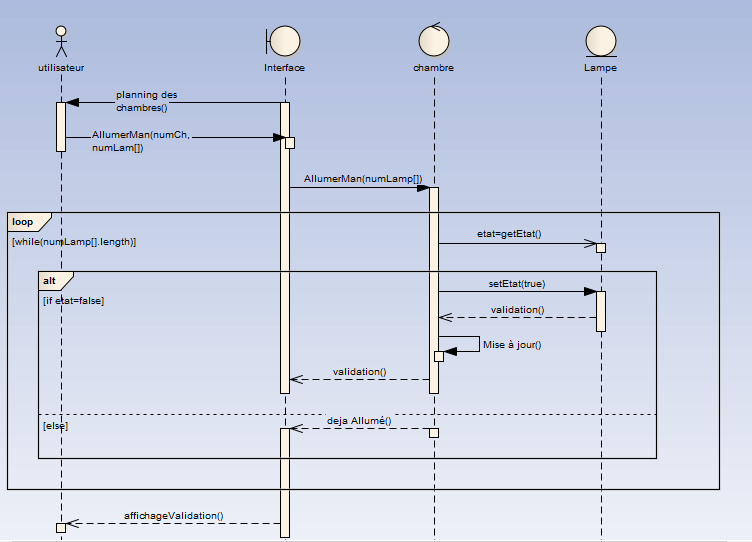
\includegraphics[scale=0.9]{15.png}
\caption{Diagramme de Séquence: Eclairage manuel}
\label{fig:fig3}
\end{figure}

\newpage

\textbf{Scénario d’extinction manuel de lumière :}
\begin{figure}[H]\centering
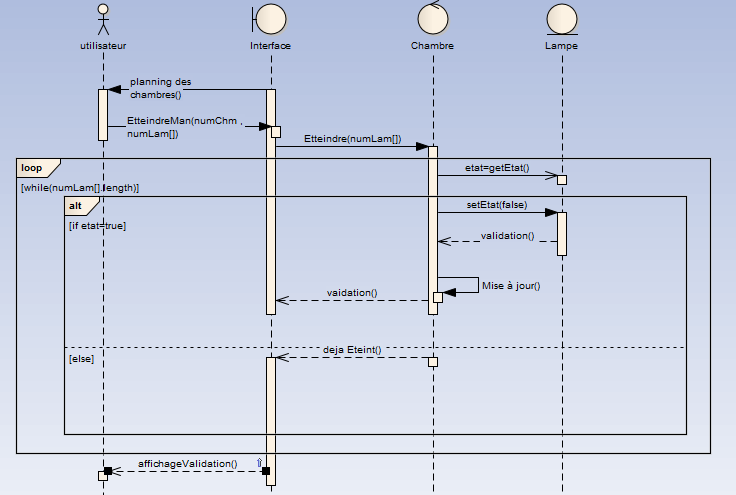
\includegraphics[scale=0.7]{16.png}
\caption{Diagramme de Séquence: Extinction manuel de lumière}
\label{fig:fig3}
\end{figure}

\newpage

\textbf{Scénario de consultation de la consommation de lumière :}
\begin{figure}[H]\centering
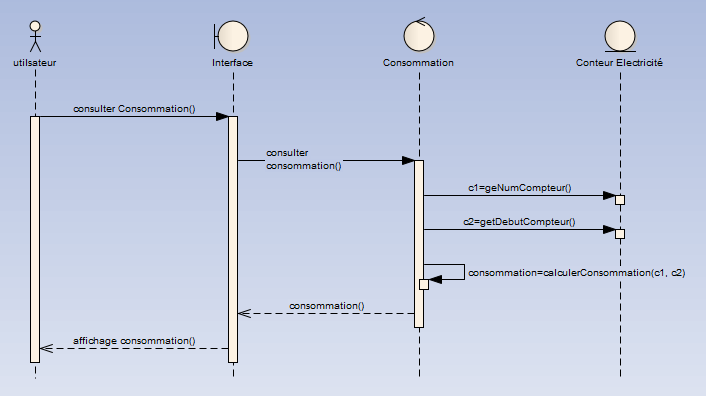
\includegraphics[scale=0.8]{17.png}
\caption{Diagramme de Séquence: Consultation de la consommation de lumière}
\label{fig:fig3}
\end{figure}
 
 
 \textbf{Scénario de réglage de degré de luminosité :}
\begin{figure}[H]\centering
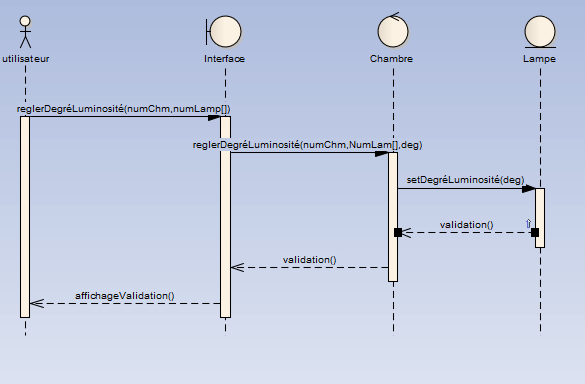
\includegraphics[scale=0.8]{18.png}
\caption{Diagramme de Séquence: Réglage de degré de luminosité}
\label{fig:fig3}
\end{figure}

\newpage
 
 \textbf{Scénario de création d’éclairage automatique :}
\begin{figure}[H]\centering
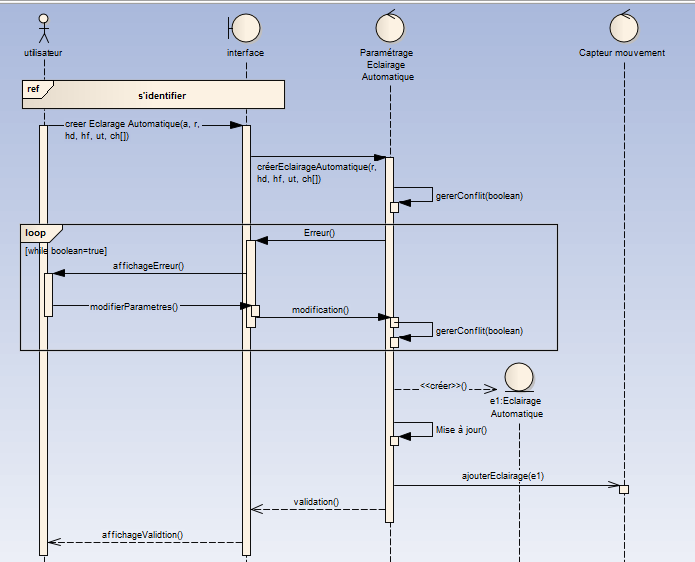
\includegraphics[scale=0.9]{19.png}
\caption{Diagramme de Séquence: Création d’éclairage automatique}
\label{fig:fig3}
\end{figure}

\newpage
 
 \textbf{Scénario de suppression d’un éclairage automatique :}
\begin{figure}[H]\centering
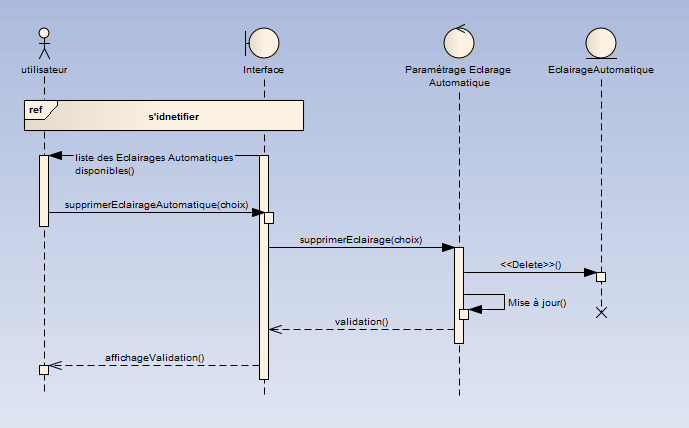
\includegraphics[scale=1]{20.png}
\caption{Diagramme de Séquence: Suppression d’un éclairage automatique}
\label{fig:fig3}
\end{figure}
 
 \newpage
 
 \textbf{Scénario de modification d’un éclairage automatique :}
\begin{figure}[H]\centering
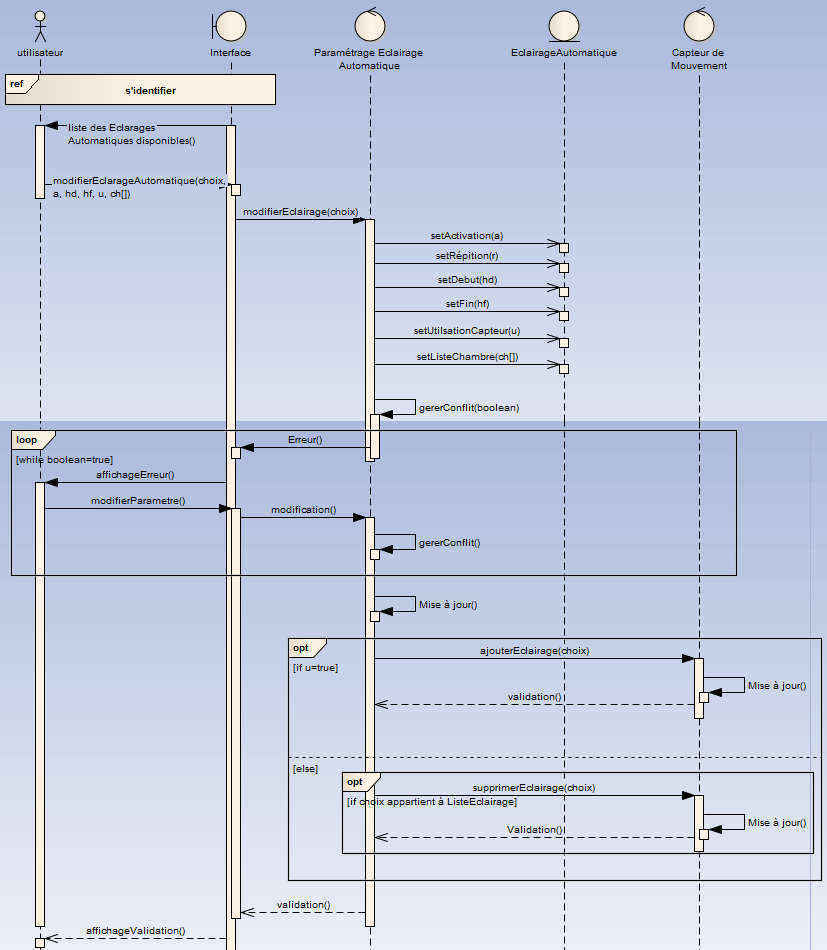
\includegraphics[scale=0.8]{23.png}
\caption{Diagramme de Séquence: Modification d’un éclairage automatique}
\label{fig:fig3}
\end{figure}
 
\subsubsection{Système des volets }

\textbf{Scénario de Fermeture des Volets :} \\
L’utilisateur peut aussi fermer manuellement les volets. lorsque l’utilisateur choisie « fermeture volet » , la liste des chambres s’affiche  ,il choisie celle qui est concerné  ainsi que  les volets qu’il veut les fermer ..si la fermeture a etteint le niveau max sans avoir toucher le bouton « stop » alors la base de donnée se mit à jours et l’etat du volet devient « fermé » sinon il reste à l’etat « ouvert » . 

\begin{figure}[H]\centering
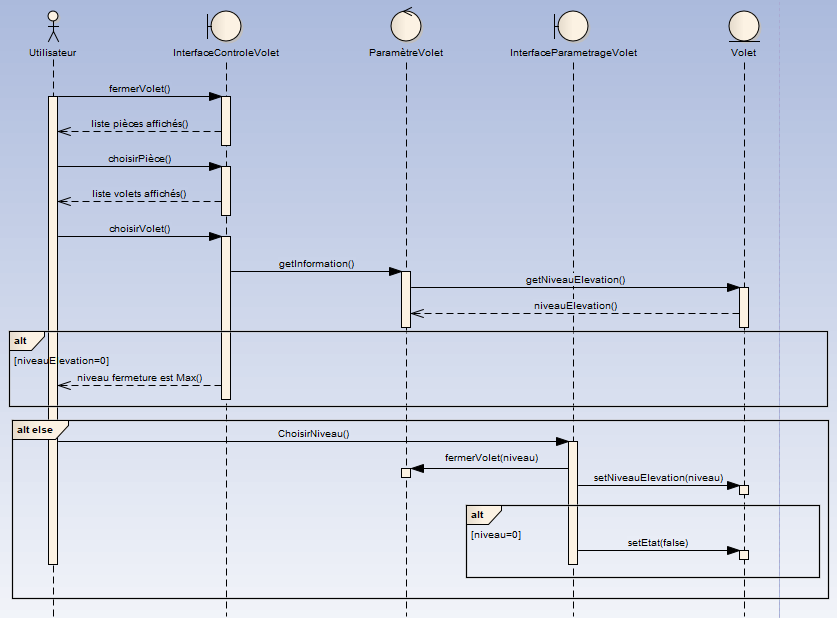
\includegraphics[scale=0.8]{24.png}
\caption{Diagramme de Séquence: Fermeture des Volets}
\label{fig:fig3}
\end{figure}

\newpage

\textbf{Scénario de Ouverture des Volets :} \\
Pour des raisons du confort , notre système assure un control à distance pour tous les volets , il suffit just d’ouvrir l’application et choisir « volet » puis « ouvrir volets » , une liste des chambres s’affiche  , l’utilisateur selectionne la chambre desiré,la liste des volets de ette chambre s’affiche,il selectionne ainsi tous les volets qu’il veut les ouvrir . apres ressemblage d’information depuis la base de donnée , un affichage du dernier etat des volets et leurs niveaux d’elevation apparait. en touchant  le bouton « ouvrir » les volets s’ouvrent jusqu’à toucher le bouton « stop » . 
\begin{figure}[H]\centering
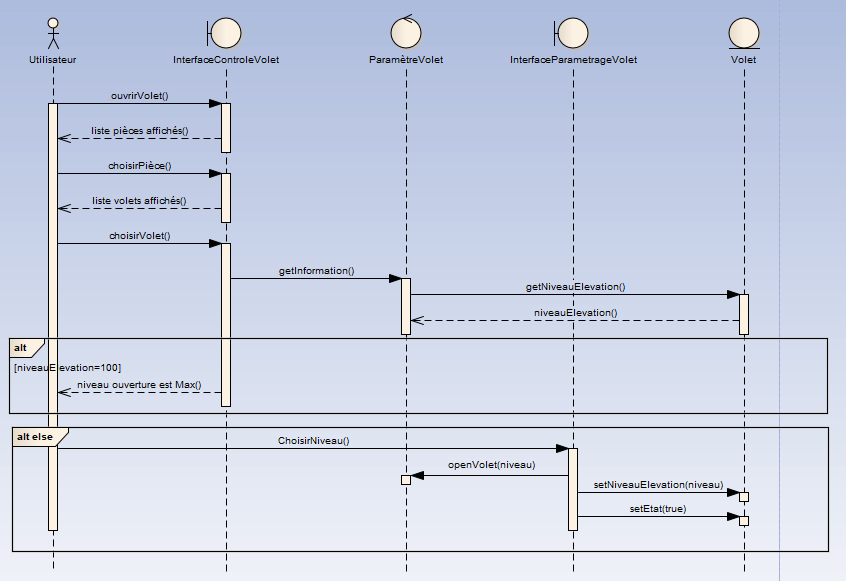
\includegraphics[scale=0.8]{25.png}
\caption{Diagramme de Séquence: Ouverture des Volets}
\label{fig:fig3}
\end{figure}

\newpage

\subsection{Diagrammes d’état-Transition}

\subsubsection{Activer/desactiver mode automatique des volets et d’arrosage Auto.}
Le système offre le choix entre l’activation ou la désactivation du mode automatique.
Il suffit juste de toucher le bouton « on/off » pour changer le mode a chaque fois.
\begin{figure}[H]\centering
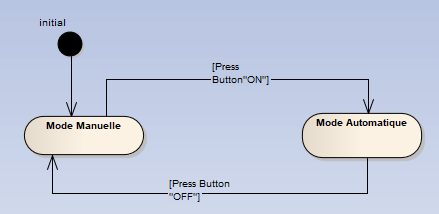
\includegraphics[scale=0.8]{26.png}
\caption{Diagramme d'état-Transition : Gestion des volets}
\label{fig:fig3}
\end{figure}

\subsubsection{Gestion des Haut-Parleurs}
\begin{figure}[H]\centering
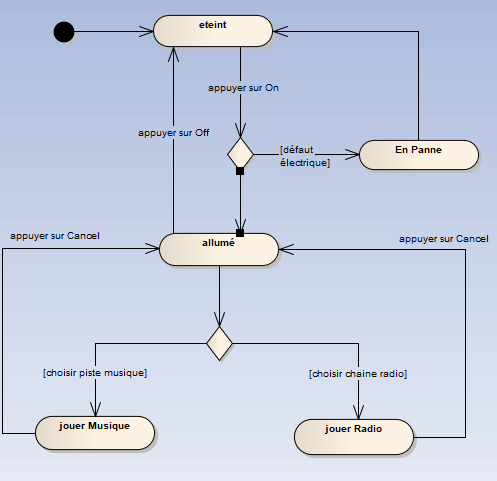
\includegraphics[scale=0.8]{27.png}
\caption{Diagramme d'état-Transition : Gestion des Haut-Parleurs}
\label{fig:fig3}
\end{figure}
 
 
 
\subsection{Diagramme d’activité }
\subsubsection{Système de caméra de surveillance }
Le vidéo de surveillance doit permettre une détection automatique de mouvement afin éventuellement de déclencher une alarme qui sera par la suite transmise vers le réseau GSM pour envoyer un SMS, ou transmise vers le réseau Wifi pour envoyer un mail pour informer l’utilisateur de ce que se passe en recevant une séquence vidéo.  

\begin{figure}[H]\centering
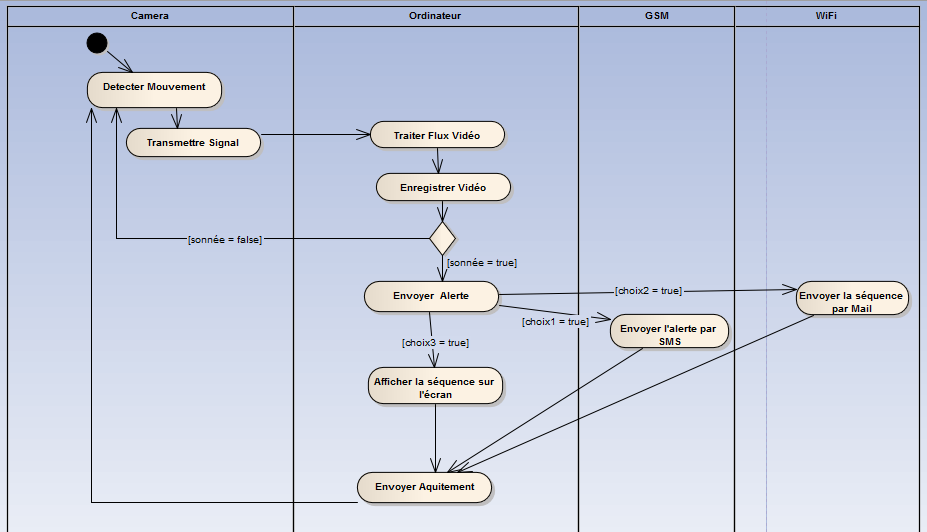
\includegraphics[scale=0.7]{28.png}
\caption{Diagramme d'Activité : Gestion des Caméras de surveillance}
\label{fig:fig3}
\end{figure}
 
 \newpage
\subsubsection{Système d’alarme d’incendie}
Cet appareil doit permettre une détection automatique d’incendie pour provoquer des actions immédiates.
En effet, un système d’alarme qui va se déclencher, avec une pulvérisation de l’eau qui reste 2 minutes puis le système envoie un SMS au pompier d’une part et aux propriétaires d’autre part. 

\begin{figure}[H]\centering
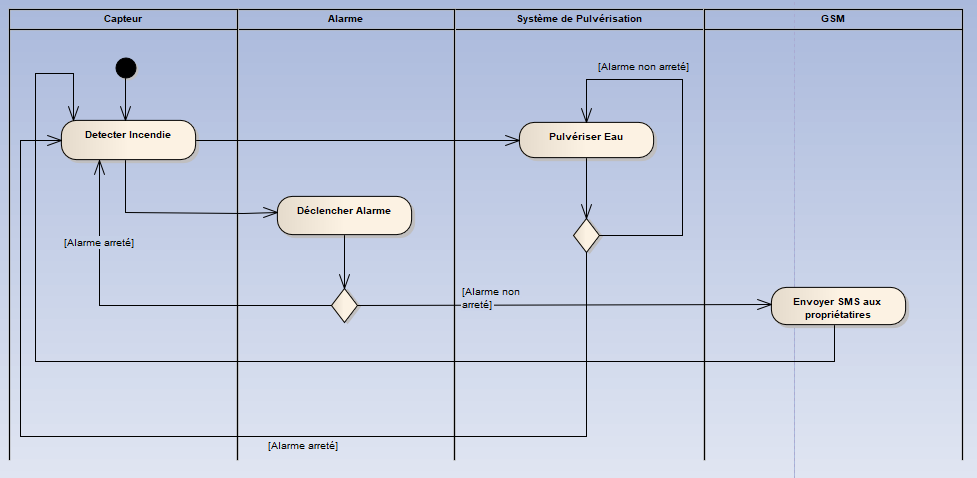
\includegraphics[scale=0.7]{29.png}
\caption{Diagramme d'Activité : Gestion d'Alarme d'incendie}
\label{fig:fig3}
\end{figure} 

\newpage
 
\subsubsection{Système d’alarme Fuite Gaz}
Cet appareil doit permettre une détection automatique d’une fuite de gaz pour provoquer des actions immédiates.
En effet, un système d’alarme qui va se déclencher puis le système envoie une notification aux propriétaires.
\begin{figure}[H]\centering
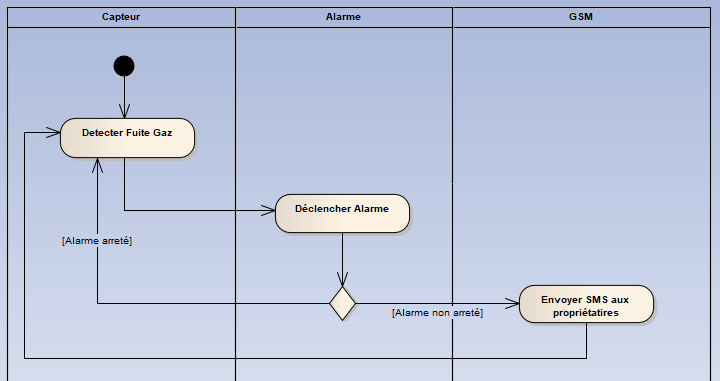
\includegraphics[scale=0.9]{30.png}
\caption{Diagramme d'Activité : Gestion d'Alarme Fuite Gaz}
\label{fig:fig3}
\end{figure} 

\subsubsection{Système d’arrosage Automatique}
\begin{figure}[H]\centering
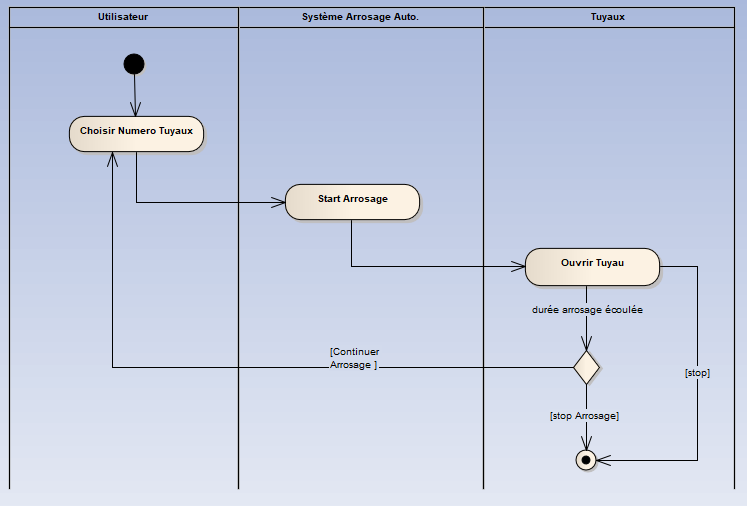
\includegraphics[scale=0.8]{31.png}
\caption{Diagramme d'Activité : Gestion d'Arrosage Automatique}
\label{fig:fig3}
\end{figure} 

\newpage

\subsection{Diagramme de Navigation}
 Permet de naviguer entre les éléments d’un système (les interfaces de l’application dans notre cas) :
 
 \begin{figure}[H]\centering
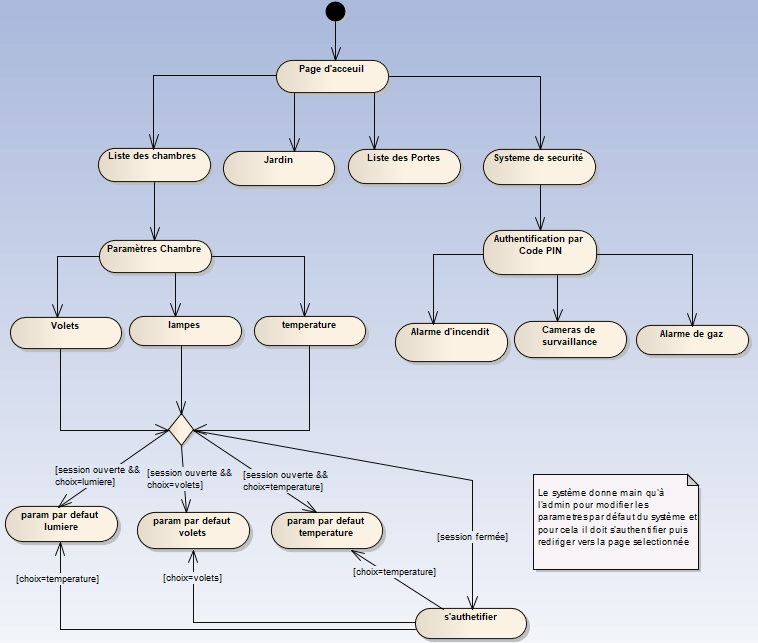
\includegraphics[scale=0.8]{33.png}
\caption{Diagramme Navigation}
\label{fig:fig3}
\end{figure} 

 
\section*{Conclusion}
Dans ce chapitre, nous avons utilisé le langage de modélisation UML (Unified Modeling Language) pour établir les différents diagrammes, ce qui nous a permis d’extraire d’une part les différentes fonctionnalités que doit offrir notre application aux différents acteurs, et d’autre part de concevoir les classes .





%==============================================================================
\end{spacing}
